\documentclass{lab}

\newcommand{\ve}[1]{\boldsymbol{#1}}

\begin{document}

\begin{titlepage}

\pagestyle{empty}	% Нумерация выкл.

\begin{center}
	\textsc{\LARGE Московский Физико-Технический Институт}\\[1,5cm]
	\textsc{\Large Кафедра общей физики}\\[0,5cm]
	\textsc{\large Лабораторная работа \textnumero 3.4.2}\\[2.5cm]

	\noindent\rule{\textwidth}{1pt}
	\\[0.5cm]
	{ \huge \bfseries Закон Кюри-Вейсса}
	\\[0.1cm]
	\noindent\rule{\textwidth}{1pt}
\end{center}

\vfill

\begin{minipage}[b]{0.3\textwidth}
	Маршрут \RomanNumeralCaps{3}\\\\
	20 октября 2018 г.\\
	27 октября 2018 г.
\end{minipage}
\hfill
\begin{minipage}[b]{0.33\textwidth}
	\textit{Работу выполнил}\\
	Ринат Валиев, 711 гр.\\\\
	\textit{Под руководством}\\
	Г.И. Лапушкина, к.ф.-м.н.
\end{minipage}

\end{titlepage}

\pagestyle{VR}
\setcounter{page}{2}

\section*{Подготовка к работе}

\subsection*{Цель работы}

Измерение подвижности и концентрации носителей заряда в металлах.

Изучение эффекта Холла.

\subsection*{Теоретическая часть}

\begin{wrapfigure}{r}{0.3\textwidth}
	\vspace{-1cm}
	\centering
	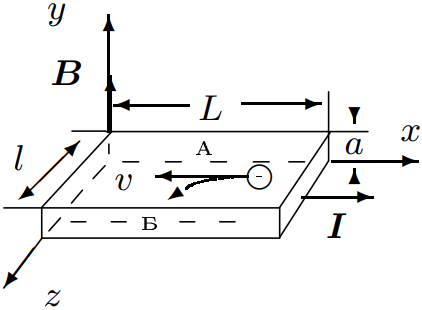
\includegraphics[width=5cm]{image1}
	\vspace{-0.7cm}
	\caption{\footnotesize Образец с током в магнитном поле}
	\label{image1}
\end{wrapfigure}

В данной работе будет рассматриваться эффект Холла. Его суть состоит в следующем. Пусть через однородную
пластину металла вдоль оси $ x $ течет ток $ I $ (Рис. \ref{image1}).

Если эту пластину поместить в магнитное поле, направленное по оси $ y $, то между гранями А и Б появляется
разность потенциалов. В самом деле, на электрон, движущийся со скоростью $ \langle v \rangle $ в
электромагнитном поле, действует сила Лоренца:
\begin{equation}
\ve{F}_л = -e {\ve{E}} - e\langle{\ve{v}}\rangle \times {\ve{B}}
\end{equation}
где, как и выше, $ e $ -- абсолютная величина заряда электрона, $ \ve{E} $ -- напряженность электрического
тока, $ \ve{B} $ -- индукция магнитного поля. В нашем случае сила, обусловленная вторым слагаемым,
направлена вдоль оси $ z $:
\begin{equation}
F_B = e | \langle v_x \rangle | B
\end{equation}
Здесь $ | \langle v_x \rangle | $ -- абсолютная величина дрейфовой скорости электронов вдоль оси $ x $,
возникающая под действием внешнего электрического поля.

Под действием этой силы электроны отклоняются к грани Б, заряжая ее отрицательно.
На грани А накапливаются нескомпенсированные положительные заряды.
Это приводит к возникновению электрического поля $ E_z $, направленный от А к Б,
которое действует на электроны с силой $ F_e = eE_z $, направленный против $ F_B $.
В установившемся режиме сила $ F_e $ уравновешивает $ F_B $, и накопление зарядов прекращается.
$$ E_z = | \langle v_x \rangle | B $$
$$ U_{АБ} = -E_zl = -| \langle v_x \rangle |Bl $$
В этом и состоит эффект Холла. Второе слагаемое в силе Лоренца, с которым связан эффект, часто называют "холловским".

Найдем ЭДС Холла:
$$ I = ne| \langle v_x \rangle |l\cdot a $$
$$ \mathscr{E}_x = U_{АБ} = - \dfrac{IB}{nea} = -R_x \cdot \dfrac{IB}{a}, ~~~~~~~ где ~~~ R_x = \dfrac{1}{ne} $$
Измеряя величину $ R_x $, можно по формуле найти концентрацию носителей тока $ n $, а по
знаку возникающей между гранями А и Б разности потенциалов установить характер проводимости
-- электронный или дырочный.

\newpage

\subsection*{Установка и измерения}

\textbf{Оборудование: } электромагнит с источником питания, источник постоянного тока, микровольтметр,
амперметры, милливеберметр, образцы из серебра и цинка.

\begin{figure}[H]
	\centering
	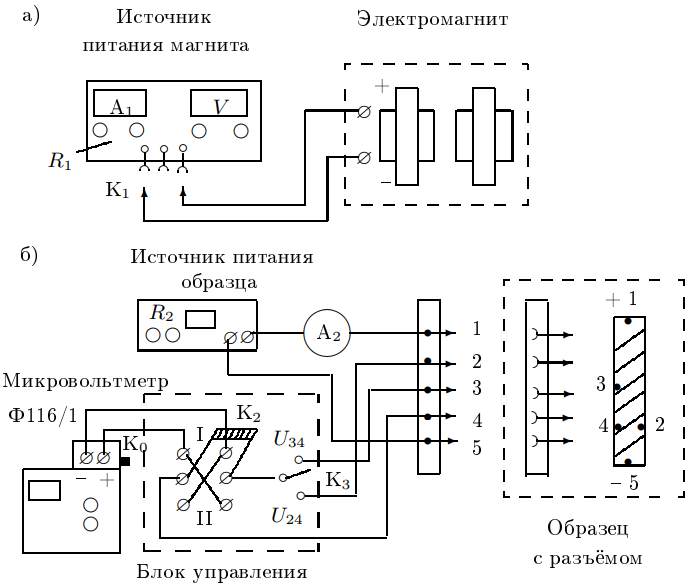
\includegraphics[width = 0.9 \textwidth]{image2}
	\caption{\footnotesize Схема установки для исследования эффекта Холла в металлах}
\end{figure}

По знаку $ \mathscr{E}_x $ можно определить характер проводимости -- электронный или дырочный. Для этого
необходимо знать направление тока в образце и направление магнитного поля.\\
Измерив ток $ I $ в образце и напряжение $ U_{34} $ между контактами 3 и 4 в отсутствие
магнитного поля, можно, зная параметры образца, рассчитать проводимость материала образца по очевидной формуле:
\begin{equation}
\sigma = \dfrac{IL_{34}}{U_{34}al}
\end{equation}
где $ L_{34} $ -- расстояние между контактами 3 и 4, $ a $ -- толщина образца, $ l $ -- его ширина.

\newpage

\section*{Ход работы}

\begin{itemize}
\item
Прокалибруем электромагнит:
\begin{table}[H]
	\centering
	\renewcommand{\arraystretch}{1.3}
%	\resizebox{0.9\textwidth}{!}{
		\begin{tabular}{|c|cccccccccc|}
			\hline
			$ I, А $	& 0.10	& 0.20	& 0.30	& 0.40	& 0.50	& 0.60	& 0.74	& 0.86	& 0.99	& 1.29\\ \hline
			$ B, мТл $	& 147	& 260	& 391	& 523	& 637	& 744	& 889	& 965	& 1028	& 1125\\ \hline
	\end{tabular}
%	}
	\renewcommand{\arraystretch}{1}
	\caption{\footnotesize Калибровка электромагнита}
	\label{tab1}
\end{table}

\item
Параметры образцов:
\begin{table}[H]
	\centering
	\renewcommand{\arraystretch}{1.3}
%	\resizebox{0.4\textwidth}{!}{
		\begin{tabular}{|c|ccc|}
			\hline
						& $ L_{34}, мм $	& $ a, мм $	& $ l, мм $ \\ \hline
			$ Цинк $	& 4		& 0.08		& 10 \\ \hline
			$ Серебро $	& 14.5	& 0.09		& 10 \\ \hline
	\end{tabular}
%	}
	\renewcommand{\arraystretch}{1}
	\caption{\footnotesize Характеристики образцов}
	\label{tab0}
\end{table}

\item
Построим график зависимости $ B(I) $ при калибровке электромагнита:

\begin{figure}[H]
	\centering
	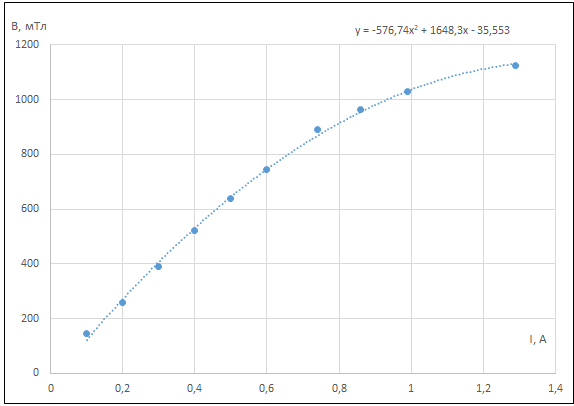
\includegraphics[width = 0.9 \textwidth]{graph1}
	\caption{\footnotesize Зависимость $ B(I) $ для таблицы \ref{tab0}}
\end{figure}

\newpage

\item
Проведем измерения ЭДС Холла. Каждый раз будем измерять начальный $ U_0 $, который вызван
несовершенством контактов 2, 4 и при фиксированном токе через образец остается неизменным.
Значение $ U_0 $ с учетом знака следует принимать за нулевое.

Измерения проводим для серебра и цинка в обратном направлении.

\begin{table}[H]
	\centering
	\renewcommand{\arraystretch}{1.3}
{
	\footnotesize
\begin{tabular}{|c|cccccccc|}
	\hline
	Серебро 				& \multicolumn{8}{c|}{$ U_0 = 0~мкВ, ~~~~~~~ I = 0.2~А $} 		\\ \hline
	$ I,~А $				& 0,20	& 0,36	& 0,43	& 0,55	& 0,64	& 0,78	& 0,96	& 1,25	\\ \hline
	$ U,~мкВ $				& 0,8	& 1,2	& 1,4	& 1,6	& 2		& 2,2	& 2,4	& 2,6	\\ \hline
	$ \mathscr{E}_x,~мкВ $	& 8		& 12	& 14	& 16	& 20	& 22	& 24	& 26	\\ \hline
	$ B,~мТл $				& 271	& 483	& 567	& 697	& 783	& 899	& 1015	& 1124	\\ \hline
\end{tabular}
\\[0.1cm]
\begin{tabular}{|c|ccccccccc|}
	\hline
	Серебро 				& \multicolumn{9}{c|}{$ U_0 = -8~мкВ, ~~~~~~~ I = 0.4~А $} 				\\ \hline
	$ I,~А $				& 0,20	& 0,36	& 0,45	& 0,57	& 0,70	& 0,80	& 0,93	& 1,05	& 1,20	\\ \hline
	$ U,~мкВ $				& 4		& 10	& 14	& 20	& 26	& 30	& 34	& 36	& 38	\\ \hline
	$ \mathscr{E}_x,~мкВ $	& 12	& 18	& 22	& 28	& 34	& 38	& 42	& 44	& 46	\\ \hline
	$ B,~мТл $				& 271	& 483	& 589	& 717	& 836	& 914	& 999	& 1059	& 1112	\\ \hline
\end{tabular}
\\[0.1cm]
\begin{tabular}{|c|ccccccc|}
	\hline
	Серебро					& \multicolumn{7}{c|}{$ U_0 = -12~мкВ, ~~~~~~~ I = 0.6~А $} \\ \hline
	$I, А$					& 0,21	& 0,39	& 0,60	& 0,80	& 1,00	& 1,20	& 1,24		\\ \hline
	$U, мкВ$				& -6	& 8		& 24	& 36	& 44	& 48	& 52		\\ \hline
	$\mathscr{E}_x, мкВ$	& 6		& 20	& 36	& 48	& 56	& 60	& 64		\\ \hline
	$B, мТл$				& 285	& 520	& 746	& 914	& 1036	& 1112	& 1122		\\ \hline
\end{tabular}
\\[0.1cm]
\begin{tabular}{|c|ccccccc|}
	\hline
	Серебро					& \multicolumn{7}{c|}{$ U_0 = -28~мкВ, ~~~~~~~ I = 0.8~А $}	\\ \hline
	$I, А$					& 0,20	& 0,40	& 0,60	& 0,80	& 1,00	& 1,20	& 1,24		\\ \hline
	$U, мкВ$				& -8	& 12	& 32	& 52	& 60	& 68	& 70		\\ \hline
	$\mathscr{E}_x, мкВ$	& 20	& 40	& 60	& 80	& 88	& 96	& 98		\\ \hline
	$B, мТл$				& 271	& 531	& 746	& 914	& 1036	& 1112	& 1122		\\ \hline
\end{tabular}
\\[0.1cm]
\begin{tabular}{|c|ccccccc|}
	\hline
	Серебро					& \multicolumn{7}{c|}{$ U_0 = -28~мкВ, ~~~~~~~ I = 1~А $}	\\ \hline
	$I, А$					& 0,20	& 0,40	& 0,61	& 0,81	& 1,00	& 1,20	& 1,25		\\ \hline
	$U, мкВ$				& -4	& 24	& 48	& 68	& 80	& 88	& 92		\\ \hline
	$\mathscr{E}_x, мкВ$	& 24	& 52	& 76	& 96	& 108	& 116	& 120		\\ \hline
	$B, мТл$				& 271	& 531	& 755	& 921	& 1036	& 1112	& 1124		\\ \hline
\end{tabular}
\\[0.1cm]
\begin{tabular}{|c|ccccccc|}
	\hline
	Серебро					& \multicolumn{7}{c|}{$ U_0 = -32~мкВ, ~~~~~~~ I = -1~А $}	\\ \hline
	$I, А$					& 0,20	& 0,40	& 0,60	& 0,80	& 1,00	& 1,19	& 1,25		\\ \hline
	$U, мкВ$				& -40	& -76	& -124	& -144	& -156	& -164	& -168		\\ \hline
	$\mathscr{E}_x, мкВ$	& -8	& -44	& -92	& -112	& -124	& -132	& -136		\\ \hline
	$B, мТл$				& 271	& 531	& 746	& 914	& 1036	& 1109	& 1124		\\ \hline
\end{tabular}
\\[0.1cm]
\begin{tabular}{|c|cccccc|}
	\hline
	Цинк					& \multicolumn{6}{c|}{$ U_0 = 72~мкВ, ~~~~~~~ I = 1~А $}	\\ \hline
	$I, А$					& 0,20	& 0,40	& 0,61	& 0,80	& 1,00	& 1,25				\\ \hline
	$U, мкВ$				& 52	& 28	& 8		& -12	& -20	& -30				\\ \hline
	$\mathscr{E}_x, мкВ$	& -20	& -44	& -64	& -84	& -92	& -102				\\ \hline
	$B, мТл$				& 271	& 531	& 755	& 914	& 1036	& 1124				\\ \hline
\end{tabular}
}
	\caption{\footnotesize Полученные данные для нахождения ЭДС Холла в образцах из серебра и цинка}
	\label{tabBig}
	\renewcommand{\arraystretch}{1}
\end{table}

\item
Определим тип носителей заряда по правилу левой руки.\\
Для таблиц \ref{tabBig} приведем график $ \mathscr{E}_x(B) $:

\begin{figure}[H]
	\centering
	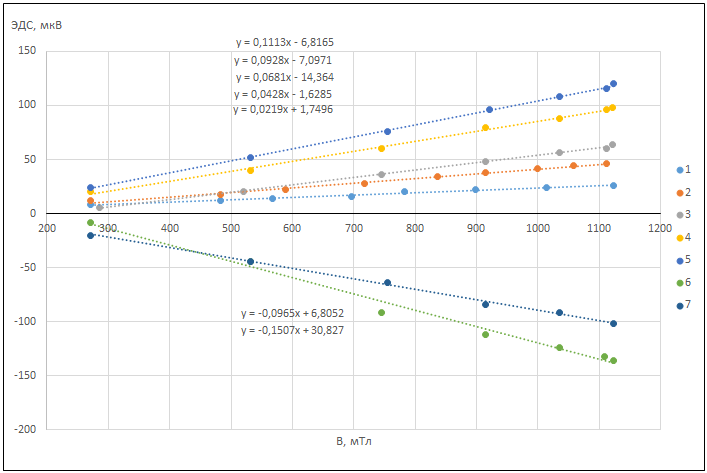
\includegraphics[width = 0.7\textwidth]{graph2}
	\caption{\footnotesize Зависимость $\mathscr{E}_x~от~B$. Данные взяты из совокупности таблиц \ref{tabBig}}
	\label{mnogo}
\end{figure}

Для каждой прямой на Рис. \ref{mnogo} найдены также их угловые коэффициенты. Внесем их в таблицу для
большей наглядности и построим по этим данным график $ k(I) $:

\begin{table}[H]
	\centering
	\renewcommand{\arraystretch}{1.3}
	%	\resizebox{0.9\textwidth}{!}{
	\begin{tabular}{|c|cccccc|}
		\hline
		$ I, А $				& 0.2	& 0.4	& 0.6	& 0.8	& 1		& -1	\\ \hline
		$ k, мкВ/Тл $			& 0.219	& 0.428 & 0.681 & 0.928 & 1.113 & -1.507	\\ \hline
		$ \Delta_k, мкВ/Тл $	& 0.2	& 0.2	& 0.2	& 0.2	& 0.3	& 0.3 \\ \hline
	\end{tabular}
	%	}
	\renewcommand{\arraystretch}{1}
	\caption{\footnotesize Таблица значений коэффициентов наклона для графика зависимости $k(I)$}
	\label{tabk}
\end{table}

\begin{figure}[H]
	\centering
	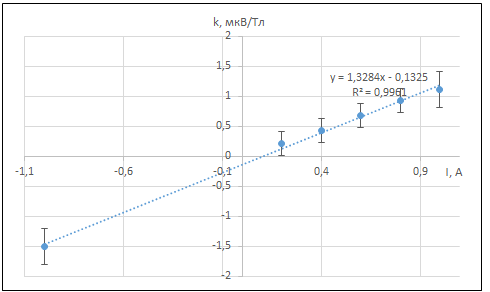
\includegraphics[width = 0.7\textwidth]{graphk}
	\caption{\footnotesize  График зависимости $k(I)$ из Таблицы \ref{tabk}}
	\label{ki}
\end{figure}

\item
По графику из Рис. \ref{ki} найдем постоянную Холла для серебра.
А для цинка определим из соответствующего графика из Рис. \ref{mnogo}.

\begin{equation}
\begin{aligned}
	&R_{серебро} = -ka = - 1.3284 \cdot 10^{-6} \cdot 0.09 \cdot 10^{-3} = -1.2 \cdot 10^{-10} м^3/Кл\\
	&R_{цинк} = - \dfrac{\mathscr{E}_{цинк}}{B} \dfrac{a}{I} = 0.965 \cdot 10^{-6} \cdot 0.08 \cdot 10^{-3} = 0.8 \cdot 10^{-10} м^3/Кл
\end{aligned}
\end{equation}

Также найдем для каждого образца концентрацию носителей заряда:

\begin{equation}
\begin{aligned}
	&n_{серебро} = \dfrac{1}{R_{серебро}e} = 5.2 \cdot 10^{28}~(м^{3})^{-1}\\
	&n_{цинк} = \dfrac{1}{R_{цинк}e} = 8.1 \cdot 10^{28}~(м^{3})^{-1}
\end{aligned}
\end{equation}

Затем заполним финальную таблицу, используя все данные и формулы:
\begin{equation}
\begin{aligned}
	&\sigma = \dfrac{IL_{34}}{U_{34}al}	&\sigma = enb\\
	&Серебро: ~~~~~ &I = 1~A, ~~~ U_{34} = 166~мкВ\\
	&Цинк: ~~~~~ 	&I = 1~A, ~~~ U_{34} = 132~мкВ\\
\end{aligned}
\end{equation}
\vspace{-0.5cm}
\begin{table}[H]
	\centering
	\renewcommand{\arraystretch}{2.1}
%	\resizebox{\textwidth}{!}{
	\begin{tabular}{|c||c|c|c|c|c|}
		\hline
		Металл	& $ R_x \pm \Delta R_x $	& Носитель	& $ n \pm \Delta n,~(м^{3})^{-1} $	
			& $ \sigma \pm \Delta \sigma,~(Ом \cdot м)^{-1} $	& $ b, \dfrac{см^2}{(В \cdot с)} $	\\ \hline
		Серебро	& $-1.2 \pm 0.1$			& -			& $(5.2 \pm 1.5) \cdot 10^{28}$
			& $ (9.7 \pm 0.8) \cdot 10^7 $						& $117 \pm 13$ 						\\ \hline
		Цинк	& $+0.8 \pm 0.2$			& +			& $(8.1 \pm 2) \cdot 10^{28}$
			& $ (3.4 \pm 0.3) \cdot 10^7 $						& $25 \pm 6$ 						\\ \hline
	\end{tabular}
%	}
	\renewcommand{\arraystretch}{1}
	\caption{\footnotesize Финальная таблица с результатами для обеих образцов}
	\label{tabfinal}
\end{table}
\vspace{-0.5cm}
\begin{table}[H]
	\centering
	\renewcommand{\arraystretch}{2.1}
%	\resizebox{\textwidth}{!}{
		\begin{tabular}{|c||c|c|c|}
			\hline
			Металл	& $ R_{табл}, \dfrac{10^{-10}~м^3}{Кл} $	& $ \sigma,~(Ом \cdot м)^{-1} $	& $ b, \dfrac{см^2}{(В \cdot с)} $	\\ \hline
			Серебро	& $-0.90$									& $6.25 \cdot 10^7$				& 56								\\ \hline
			Цинк	& $+1.04$									& $1.7 \cdot 10^7$				& 17.5 								\\ \hline
		\end{tabular}
%	}
	\renewcommand{\arraystretch}{1}
	\caption{\footnotesize Табличные данные для сравнивания с результатами}
	\label{tabl}
\end{table}

\end{itemize}

\subsection*{Итоги}

В работе исследован эффект Холла в металлах, найдены некоторые характеристики для образцов из разных
материалов. Некоторые табличные данные не совпадают с результатами нашей работы, однако они достаточно
точно описывают характеристики образцов.\\
Также установили знак носителей зарядов в данных образцах металлов.


\end{document}